
%Reasons for only searching ``search'' visits:
%Using info that depends on a presence of a SN will create a bias. 
%Also, we don't want to consider supernovae found in the last visit to
%a cluster, as it would be very difficult to determine the type of a SN
%based on only one light curve point on the rise.

For the purpose of initially detecting candidates, we use only
``search'' visits (filled circles in Fig.~\ref{fig:visits}) and
disregard the ``follow-up'' visits (open circles in
Fig.~\ref{fig:visits}). (In the following section we will use any
available ``follow-up'' visits to construct more complete light curves
for the candidates discovered in this section.) We use the {\sc
MultiDrizzle}-combined, cosmic ray-rejected, $z_{850}$ image from each
``search'' visit. We consider only regions in this image that are
covered by three or more $z_{850}$ exposures.  With less than three
exposures, the combined images are too heavily contaminated by cosmic
rays to be practically searchable for SNe. Although there are
typically four $z_{850}$ exposures, the dither pattern used in the
survey means that not all regions of the combined image have four
exposures. The ACS camera is a mosaic of two $2048 \times 4096$~pixel
CCD chips (1~pixel = $0.05''$) separated by $2.5''$. The $z_{850}$
exposures were dithered to cover this gap, meaning that a $5''$ wide
region in the center of the image and $2.5''$ wide regions on either
side of the image are only covered by two exposures and thus are not
searchable. Due to orbital constraints, the position angle of {\it HST}
changes between each visit. This means that the unsearchable ``gap''
region rotates over the field between visits, and that the outer parts
of the field are observed in some visits, but not others
(Fig.~\ref{fig:epochs}, second row). The regions around bright stars
are also considered ``not searchable'' and are similarly masked.

%%%%%%%%%%%%%%%%%%% 
% PLOT: EPOCHS    %
%%%%%%%%%%%%%%%%%%%
\begin{figure}[p]
\begin{center}
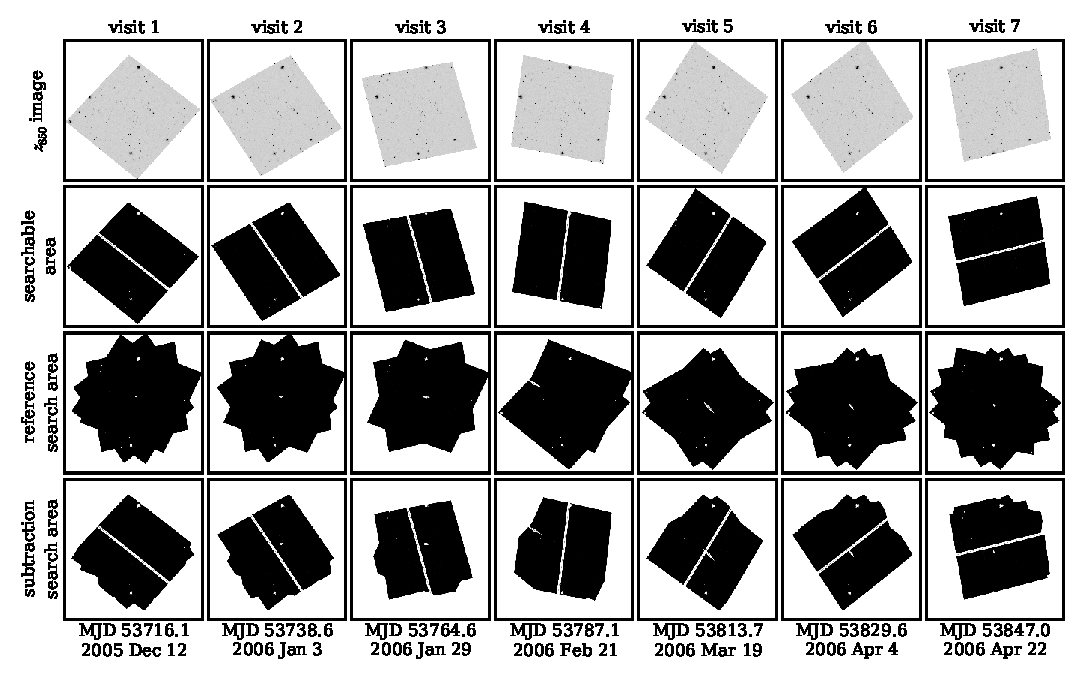
\includegraphics[width=6.75in,angle=270]{figures/cands/epochs.eps}
\end{center}
\caption[An example of image orientation and searchable regions]
{An example of image orientation and searchable regions for cluster
ISCS J1432.4+3332. Each column represents an observation of the
cluster. The first row is the $z_{850}$ image for that visit. The
second row is the part of that image that is searchable. The third row
shows the searchable area of the stacked reference image used in the
subtraction for this visit. The fourth row is the searchable area in
the subtraction (the intersection of the second and third
rows).  \label{fig:epochs}}
\end{figure}

For each ``search'' visit to each cluster, we follow these four steps:
\begin{enumerate}
\item {\bf A reference image is made} by combining images from
other visits to the cluster. All visits that are either 50 or more
days before the search epoch or 80 or more days after the search epoch
are included. If there are no epochs outside this 130~day range, the
range is narrowed symmetrically until one epoch qualifies. Masked
pixels in each visit's image do not contribute to the stacked
reference image (Fig.~\ref{fig:epochs}, third row).

\item {\bf A subtracted image is made} by subtracting the stacked
reference image from the search epoch image. A map of the sky noise
level in the subtraction is made by considering the noise level of the
search epoch image and the noise level of each reference image
contributing to a given region. Any area masked in either the search
epoch or stacked reference image is masked in the subtracted image
(Fig.~\ref{fig:epochs}, fourth row).

\item {\bf Candidates in the subtraction are identified by software.} To
  be flagged, a candidate must have three contiguous pixels with a flux
  3.4 times the local sky noise level in the subtraction (as
  determined by the sky noise map above). Once flagged, it must
  fulfill the following four requirements:
\begin{itemize}
\item {\sc MultiDrizzle}-combined image: A total signal-to-noise ratio 
  (including sky and Poisson noise) of 5 or more in a 3~pixel radius
  aperture.
\item {\sc MultiDrizzle}-combined image: A total signal-to-noise ratio 
  of 1.5 or more in a 10~pixel radius aperture.
\item Individual exposures: A signal-to-noise ratio of 1 or greater 
  in a 3~pixel radius aperture in three or more individual exposures.
\item Individual exposures: A candidate cannot have an individual exposure 
  with a flux more than $20\sigma$ greater than the flux in the lowest 
  flux exposure \emph{and} a second individual exposure with flux more 
  than $10\sigma$ greater than the flux in the lowest flux exposure.
\end{itemize}
The first requirement is designed to eliminate low significance
detections on bright galaxies. The second requirement helps eliminate
dipoles on bright galaxy cores caused by slight image misalignment. The
third and fourth requirements are aimed at false detections due to
cosmic ray coincidence. They require the candidate to be detected in
most of the exposures and allow no more than one exposure to be
greatly affected by a cosmic ray. On the order of five to ten
candidates per subtraction pass all the requirements, resulting in
approximately 1000 candidates automatically flagged across the 155
search visits.

\item {\bf Each candidate is evaluated by eye in the subtraction.}
Because the position angle changes between each epoch, the orientation
of stellar diffraction spikes changes, causing the majority of the
false detections. These are easy to detect and eliminate by
eye. Occasionally there are mis-subtractions on the cores of bright
galaxies that pass the above requirements. Only completely unambiguous
false detections are eliminated in this step. If there is any
possibility the candidate is a real SN, it is left in the sample for
further consideration.
\end{enumerate}

After carrying out the above four steps for all 155 search visit, 86
candidates remain. At this point, candidates have been selected based
only on information from a single $z_{850}$ subtraction.
